\chapter[Sensor de Posição Angular]{Sensor de Posição Angular}

\begin{enumerate}
  \item \textbf{Operação}

    O sistema irá ficar ativo o tempo todo, e durante todo o percurso deverá detectar quando o usuário desejar fazer uma ultrapassagem. Para isso, torna-se necessária a utilização de um sensor de rotação. Assim, sempre que o usuário rotacionar o volante X graus, o sistema entenderá que o usuário tem a intenção de fazer a ultrapassagem e começará os cálculos e operações necessárias para informar sobre a viabilidade da manobra.

    O modelo do sensor de rotação a ser utilizado varia de acordo com a marca, modelo, tipo de combustível e ano do carro. Por esse motivo, não é possível utilizar um sensor que funciona em qualquer carro. Pensando nisso, o seu uso no projeto se baseou na situação hipotética de que todos os carros já vem com o sensor embutido.

    \begin{figure}[h]
      \centering
      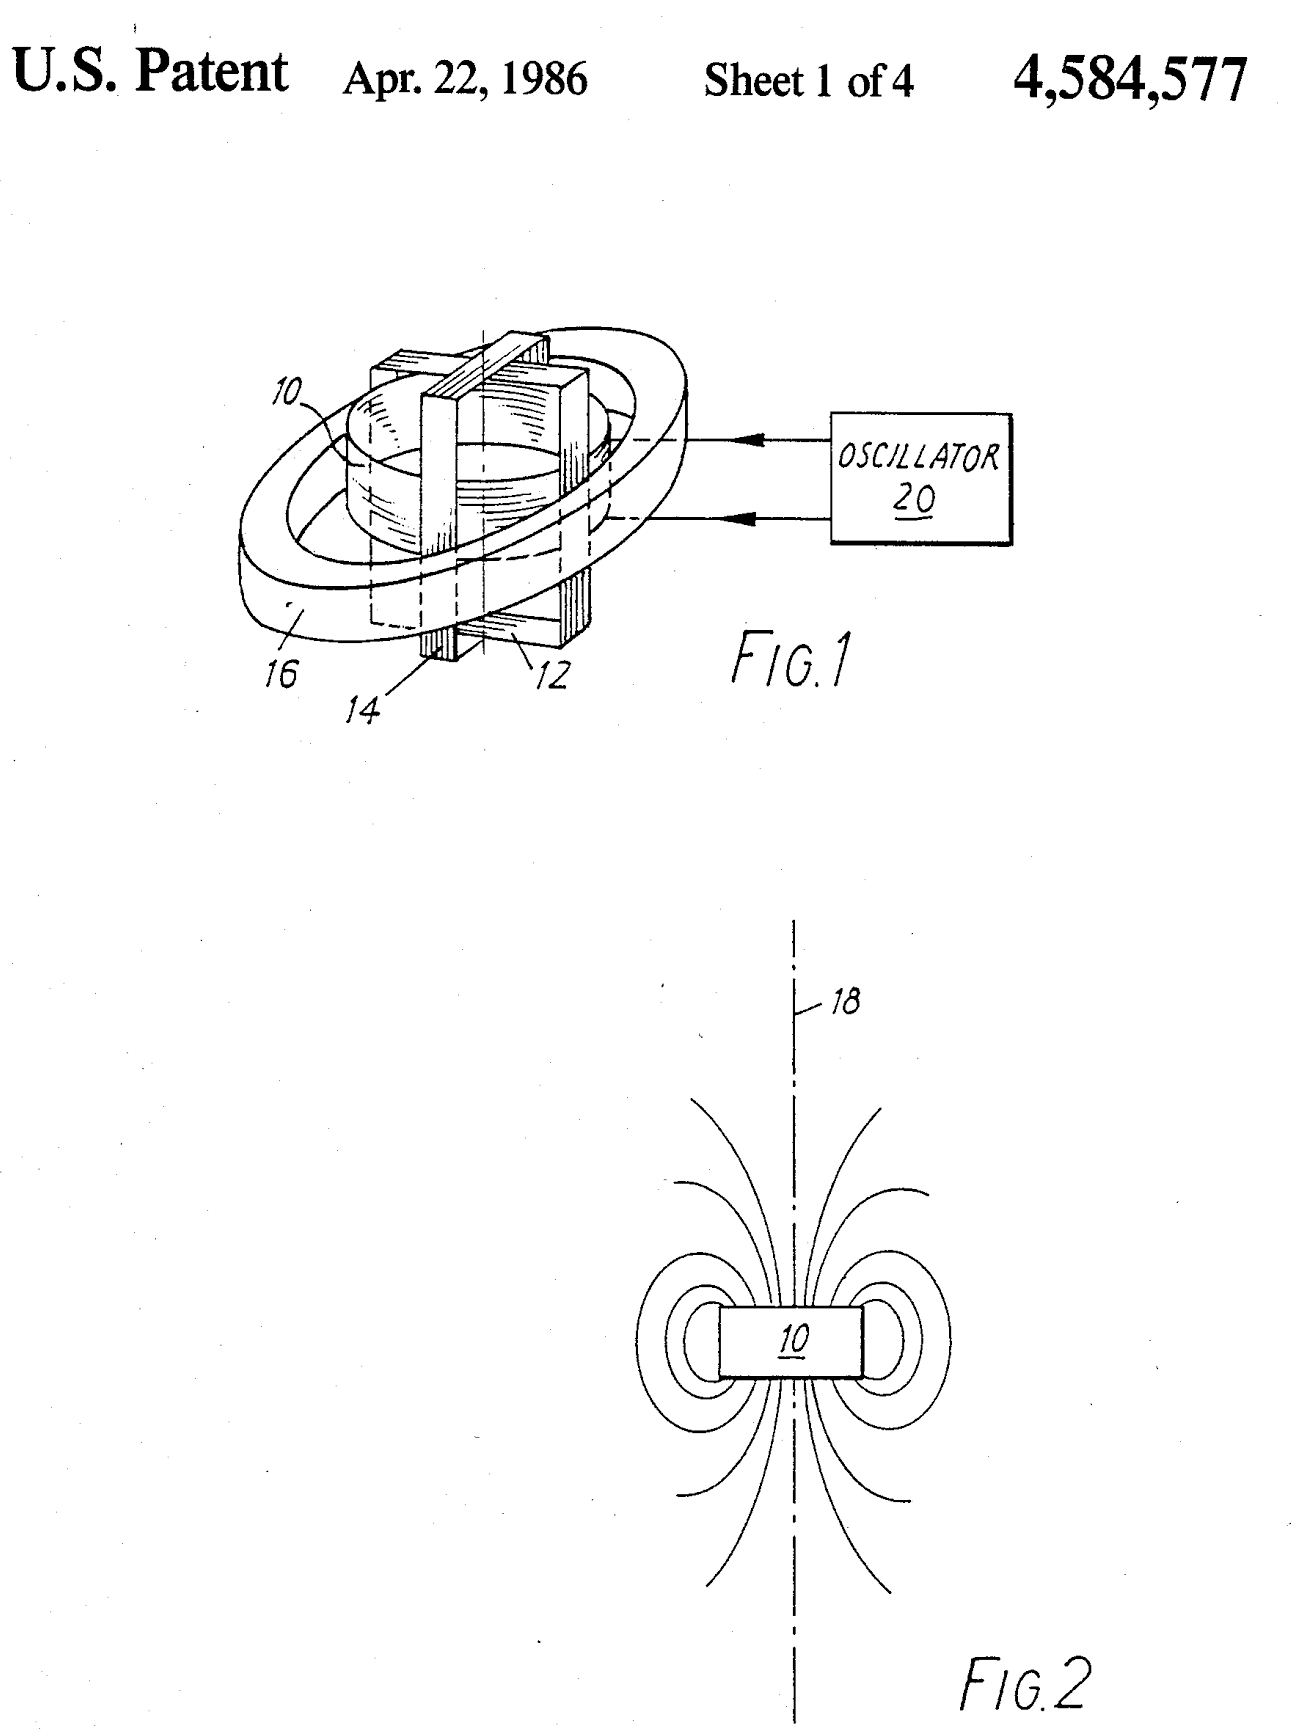
\includegraphics[height=250px, scale=0.5]{figuras/patente1}
      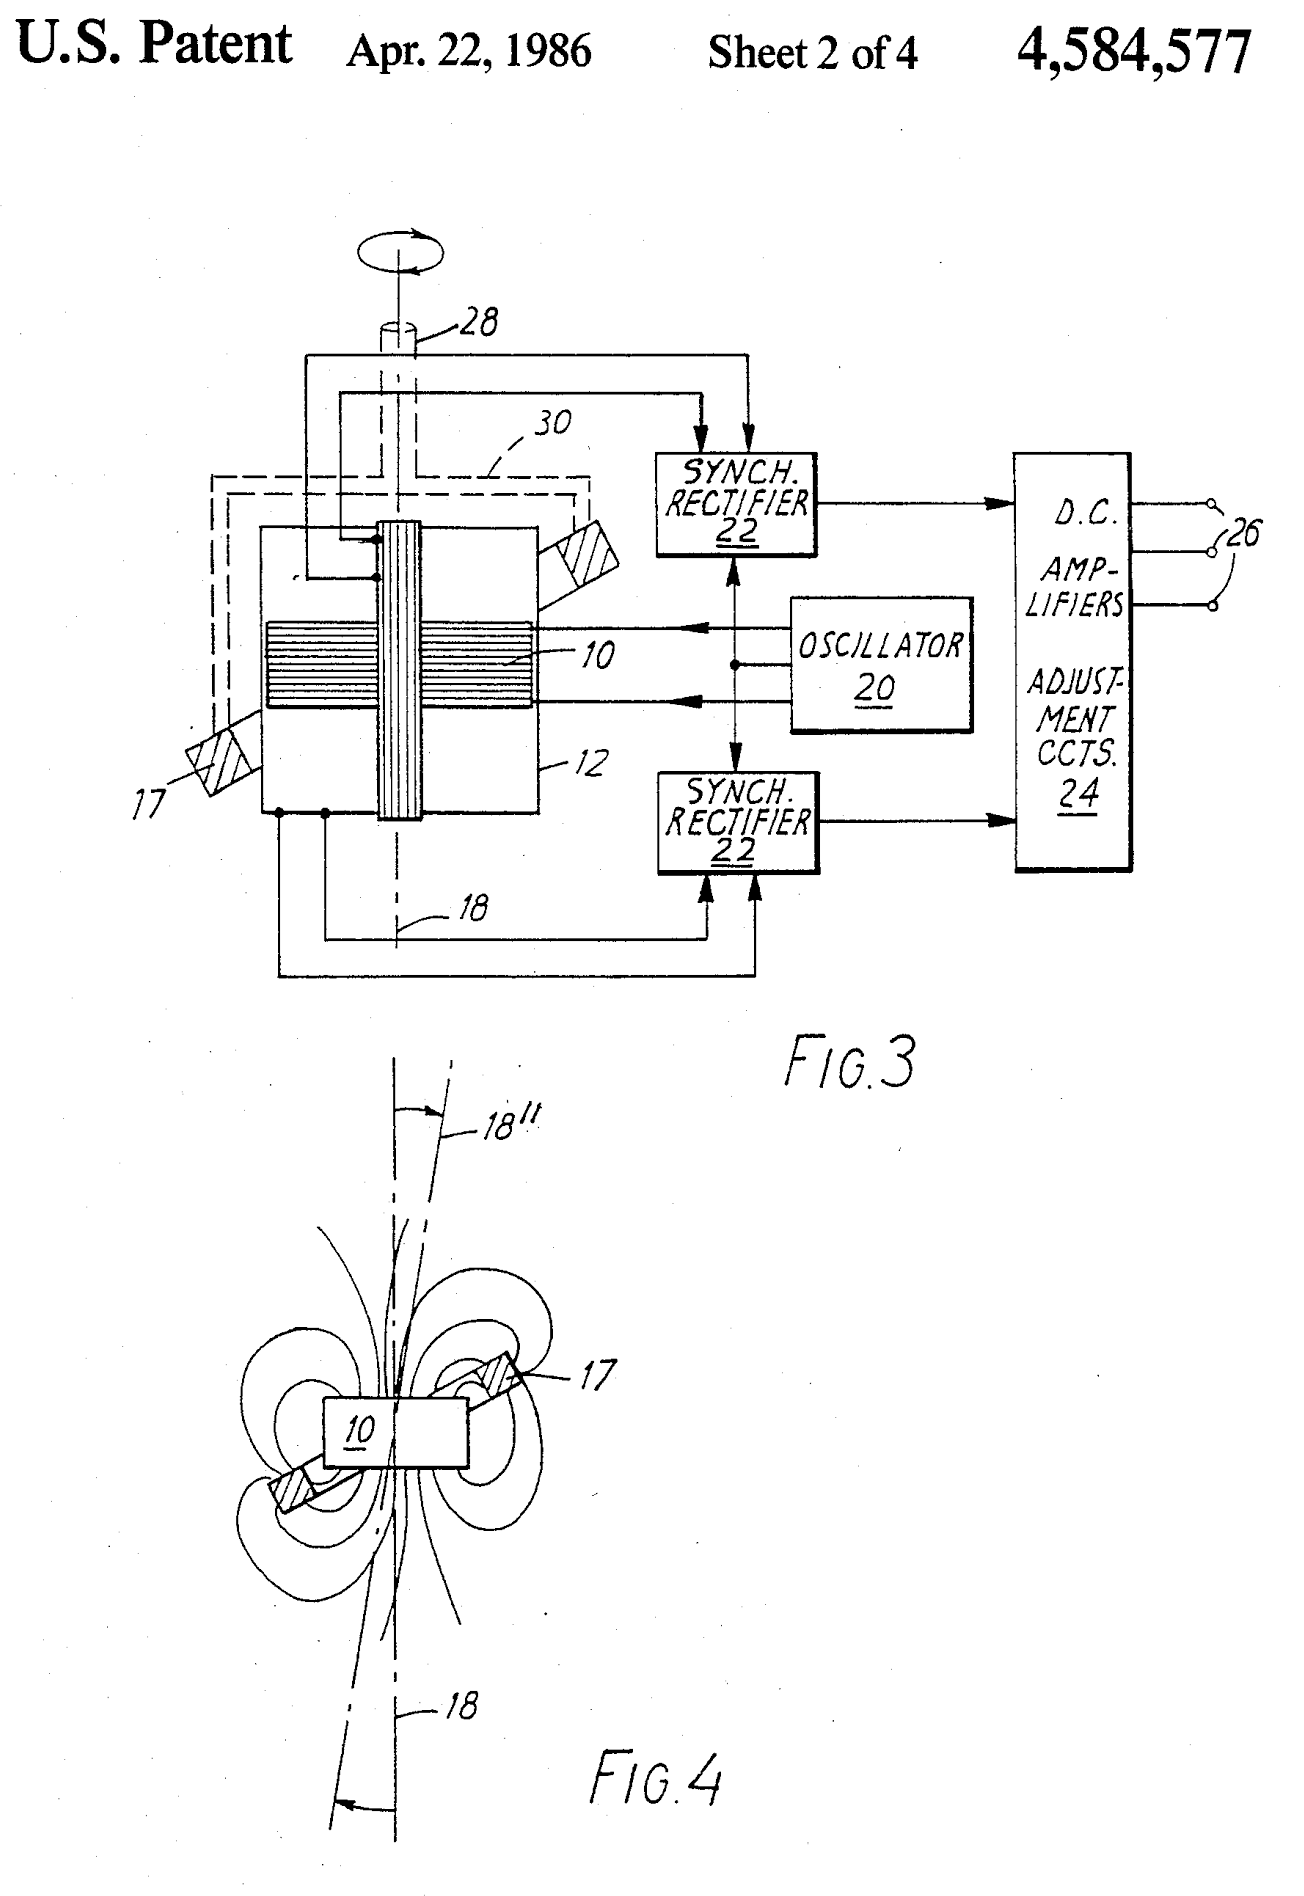
\includegraphics[height=250px, scale=0.5]{figuras/patente2}
      \label{table:patente1}
    \end{figure}

    \begin{figure}[h]
      \centering
      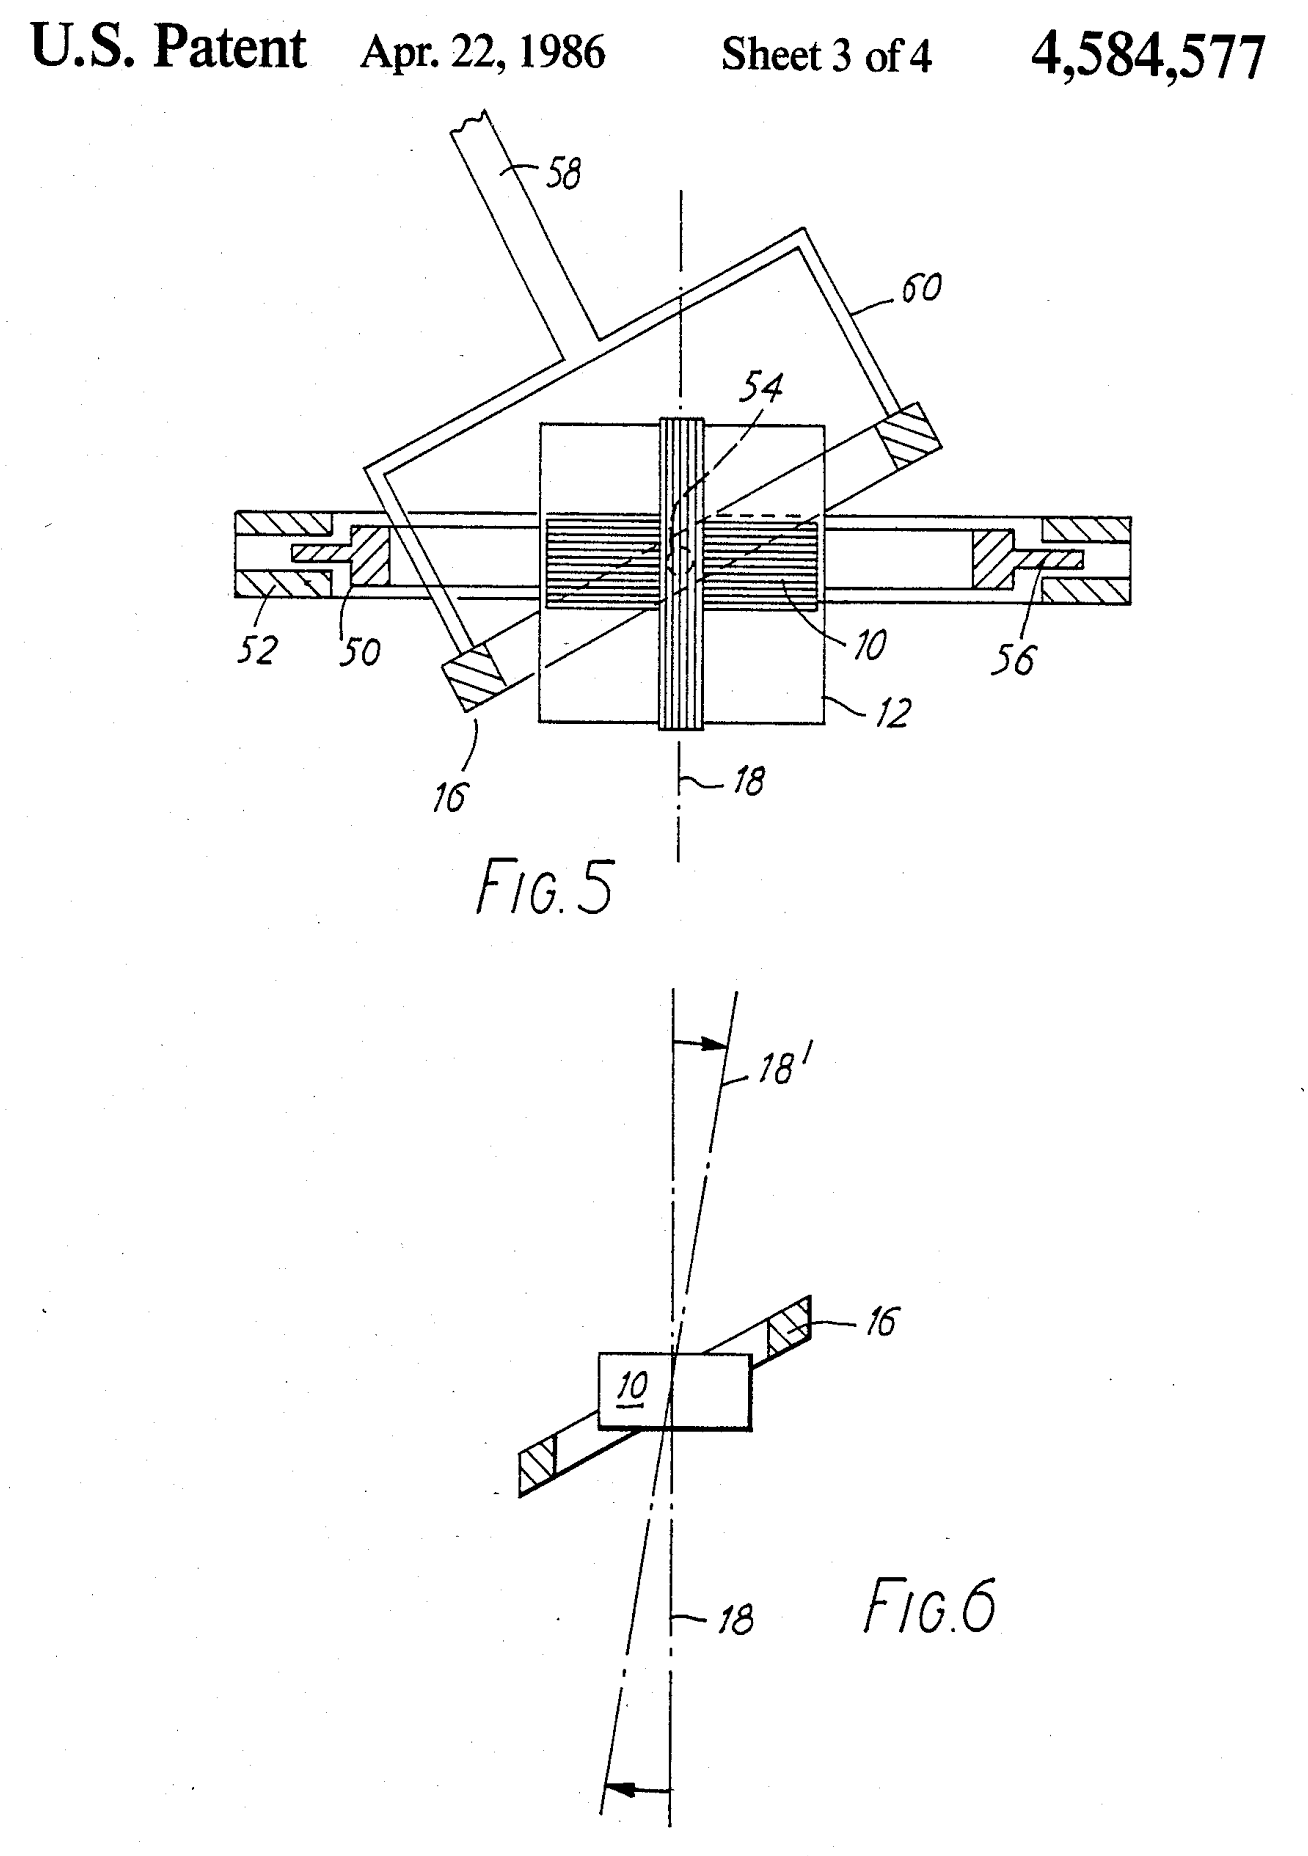
\includegraphics[height=250px, scale=0.5]{figuras/patente3}
      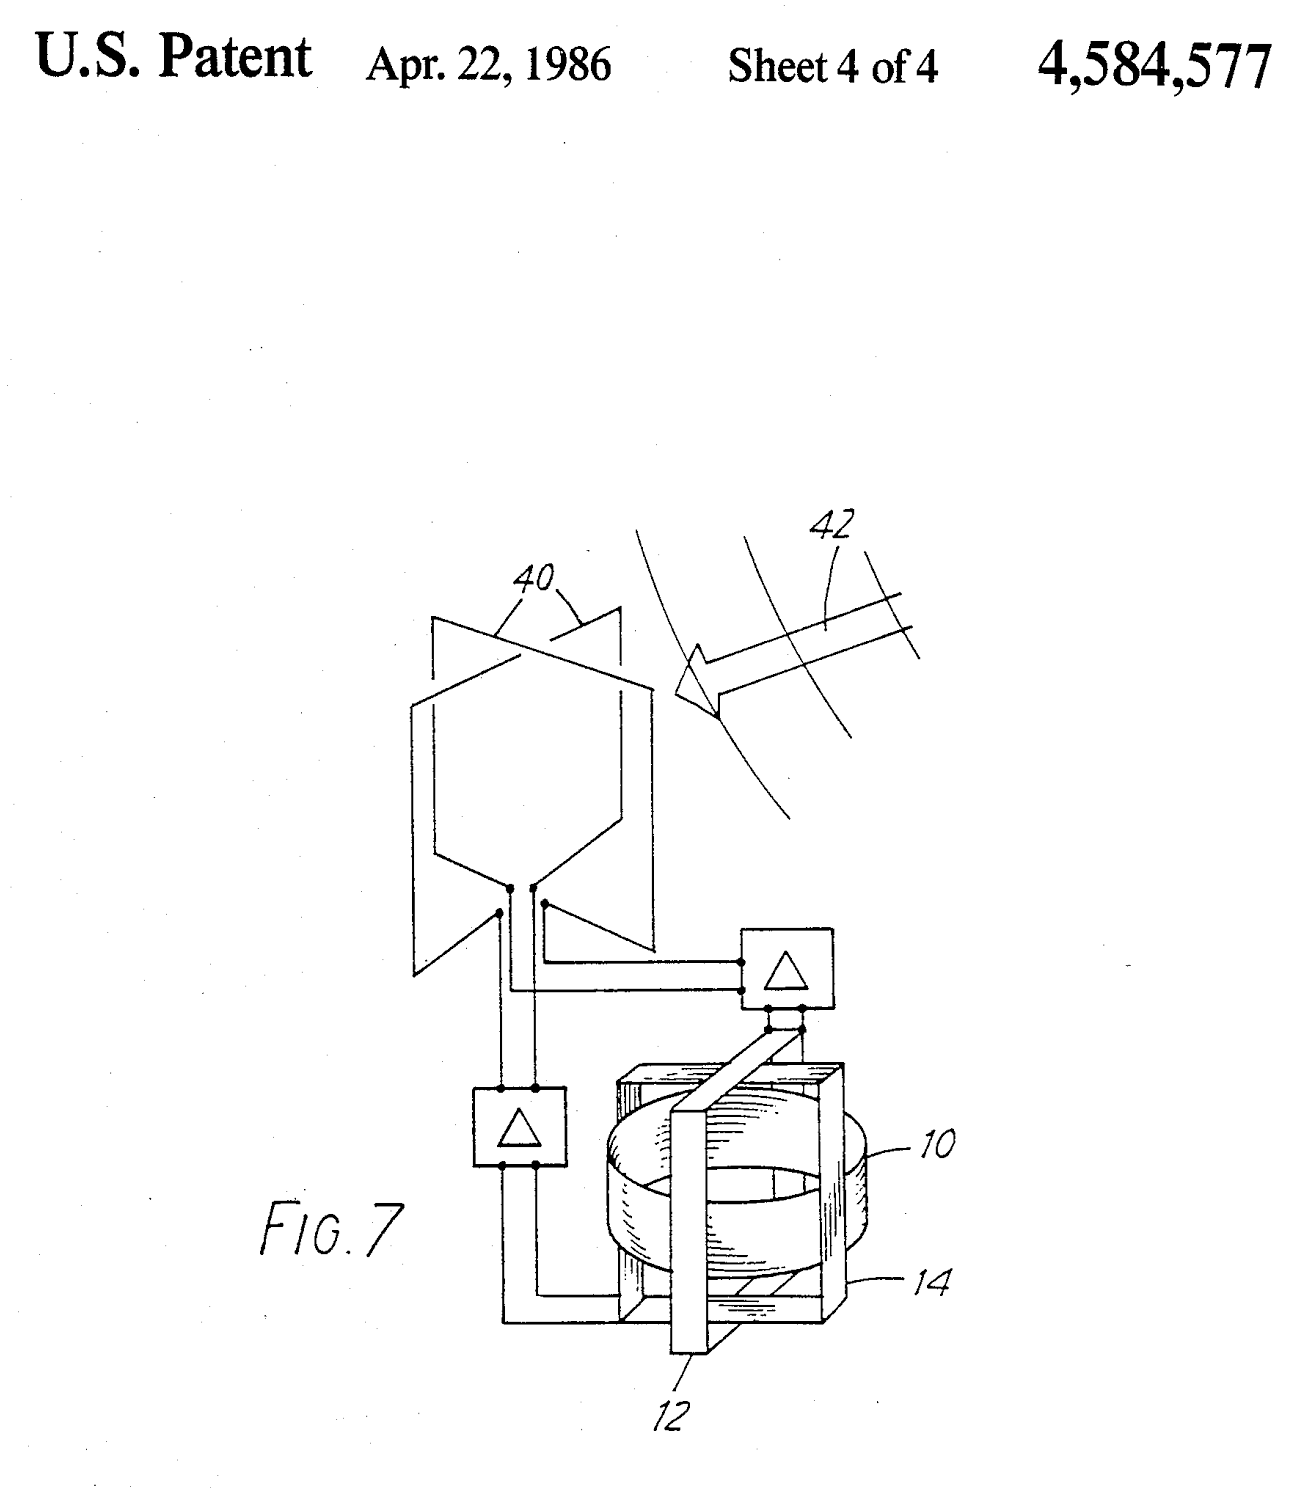
\includegraphics[height=250px, scale=0.5]{figuras/patente4}
      \label{table:patente2}
    \end{figure}

  \item \textbf{Funcionamento}

  Um sensor de posição angular funciona utilizando uma bobina para gerar um campo magnético alternado simétrico, a frequência do oscilador adequada para utilizar é de 500 KHz a vários MHz. Para o veiculo, faixas de operação de 1,6 MHz é baixa e não devem ser utilizados, pois sao feitos para circuitos simples e dispositivos pequenos.

  Na imagem 1 é visivel a bobina que gera o campo maguinético: componentes 10, 12 e 14 e o oscilador 20. Assim como há uma representação do campo gerado por estes.

  As bobinas de detecção 12 e 14 são idênticas e estão dispostas perpendicularmente entre si e em relação ao plano que contém a bobina do gerador 10. Com esta disposição, o eixo de simetria 18 da campo magnético produzido pela bobina do gerador 10 situa dentro dos planos delimitados pelas bobinas 12 e 14 e, na ausência do rotor 16, há EMF induzida na bobina de detecção quer de 12 ou 14 pelo campo magnético alternado.

  O rotor 16 tem a forma de um corpo plano, neste caso, uma coroa circular. O rotor anelar podem ser de um material magnético ou seja electricamente condutor, mas é preferível usar um rotor condutor de electricidade para a facilidade de fabrico. O rotor 16 das FIGS. 1 e 6 é formado, por exemplo, por um anel de corte a partir de um pedaço de tubo de cobre com um ângulo ao seu eixo.

  O sensor de posição mostra como a posiçao angular do sensor da invenção pode ser modificado para monitorar a posiçao angular do eixo rotatório 28, utilizando um rotor magnético 17 de ferrite ou pó de ferro. O rotor 17 é montado na extremidade do rotor 28 por meio de um Suport 30, de modo que é simetrico sobre o eixo 28 e inclicado e inclinado em relaçao ao plano da bobina do gerador 10. O rotor 28 é posicionado de modo que o seu eixo longitudinal coincida com o eixo de simetria do campo magnético de relutância mais baixa do que o ar circundante. Como resultado, o campo magnético é distorcido em torno do rotor 17, assim como mostrado na FIG. 4. O suporte 30 é de um material não magnético de modo que ela própria não provoca qualquer distorção do campo magnético.

  A medida que o eixo 28 é rotacionado, o campo magnético do rotor 17 e 18 sao distorcidos en relação a ele. O acoplamento electromagnético entre o campo magnético e as bobinas de detecção dá origem a um sinal de saída a partir de cada uma das bobinas 12 e 14, que varia à medida que o eixo 28 gira. Para se obter as posições angulares de 0º a 359º, os parâmetros físicos do dispositivo devem estar ajustados adequadamente as saídas das 12 e 14, pois através do ângulo do rotor 17 em relação ao eixo 18 é possivel determina-las.

  Como o rotor 17 executa uma unica revolução, a fase do sinal de saída em cada bobina de detecção 12 ou 14 reveses. As saídas da bobina de detecção são, portanto, aplicadas a um par de retificadores síncronos 22, que comparam a fase de cada sinal de saída da bobina de detecção com a fase de saída do oscilador 20 e produzem um sinal de corrente contínua de polaridade correta e de uma magnitude correspondente para a amplitude da bobina de detecção de saída. Os sinais de DC são então amplificados e passados através de circuitos de correção 24 para os terminais de saída 26 do dispositivo. Uma vez que os erros na saída de uma das bobinas de detecção 12 e 14 ocorram, se as bobinas 10, 12 e 14 não são precisamente relacionadas umas as outras, os circuitos de correção 24 são incluídos para fornecer correção elétrica destes erros e, assim, evitar a necessidade de um conjunto de bobinas móveis complexas. Os circuitos de correção 24 incluem meios convencionais para compensar os deslocamentos de origem que surgem quando os sensores e bobinas geradoras não são precisamente ortogonais e para ajustar a saída para ter em conta os erros nela, devido à falta de ortogonalidade entre as bobinas de detecção 12 e 14, e para uma saída não balanceada entre eles. Os circuitos de correção 24 ativam o dispositivo de detecção de posições angulares com uma precisão superior a 1º.

  A falta de ligaçao mecânica entre os eixos 28 e as bobinas 12 e 14, possibilita identificar a rotação contínua sobre aquele eixo para qualquer direção.

  A imagem 4, exibe que o dispositivo pode ser alterado para controlar a direçao de uma onda electromagnética. Nesta imagem, as bobinas estao nas mesmas posições que o da imagem 1, entretanto neste dispositivo desempenharão papel invertido. O sinal enviado por cada par de antenas e amplificada e aplicada as bobinas. As antenas 40 são perpendiculares umas as outras e sinalizam o componente do vetor em cada uma delas. Quando o dispositivo está em utilizaçao, as bobinas 12 e 14 geram campos magneticos alternados de grandeza porporcional a um componente da onda de entrada 42. Assim a direção da onda magnética resultante está relaciodada a onda de entrada 42. Quando o rotor está inclinado, o campo magnético é distorcido, de forma que ele tem uma componente numa direção perpendicular ao plano da bobina 10.

  A posição do rotor é ajustado até que a saída da bobina 10 atinja um valor nulo. A posição angular nula do roto, fornece uma indicação da direcção da onda de entrada. Assim o dispositivo pode ser utilizado para descobrir uma direção de entrada da onda.

  Com a descrição do funcionamento acima, o sensor pode ser capaz de realizar diversas funções inclusive determinar a quantidade de tempo em que o volante esta em uma determinada posição. E devido a sua construção, este poder ser robusto o suficiente para ser utilizado no projeto CIAC. E pode ser fabricado por um baixo custo por métodos convencionais.

  \item \textbf{Materiais básicos a qualquer sensor de rotação:}
  \begin{itemize}
    \item Uma bobina geradora acionável, para proporcionar um campo magnético alternado simétrico em torno de um eixo central da referida bobina do gerador;

    \item Um par de sensores dispostos de modo que o plano que contém cada bobina de detecção seja ortogonal ao plano que contém os outros meios de detecção e a bobina que contém o referido gerador de bobina;

    \item Um corpo de material condutor de eletricidade, em que pelo menos uma parte do mesmo esteja diposta no exterior dos planos contendo o gerador e o detector de bobinas seja rotacionável sobre o eixo central do dito gerador. Os campos eletromagnéticos induzidos sobre a detecção das bobinas pelo campo magnético passam a ser dependentes da posição angular do referido corpo relativo ao eixo de simetria do campo magnético não distorcido.

  \end{itemize}

  \item \textbf{Itens necessários para detecção:}

  Para realizar a detecção da posição angular ou da movimentação angular sobre um determinado eixo é necessário:

  \begin{itemize}
    \item Obter meios para gerar campo magnetico alternado e simétrico;

    \item Um corpo assimetrico sobre o eixo que se deseja obter a posiçao angular, uma parte da qual é encontrada fora do campo magnetico alternado, perpendicular ao eixo desejado;

    \item Uma bobina de detecção no interior do campo eletromagnetico resultante;

    \item A EMF induzida na bobina de detecção dependente da posição angular do campo resultante.

  \end{itemize}

  \item Para explicar o funcionamento, foi utilizado o sensor PMS-CKP (Imagem 1) como exemplo. Ele funciona nos seguintes modelos de carro:
  \begin{table}[h]
    \centering
    \begin{tabular}{llll}
    Montadora & Modelo           & Motor              & Ano                      \\
    GM        & Astra            & 1.8 MPFI           & 10/98 a 09/04            \\
    GM        & Astra            & 2.0 MPFI           & 09/94 a 09/04            \\
    GM        & Astra            & 2.0i               & 09/91 a 02/98            \\
    GM        & Astra Sedan      & 2.0 MPFI FlexPower & 10/04 a hoje             \\
    GM        & Blazer           & 2.2 MPFI           & 08/97 \textgreater 01/07 \\
    GM        & Blazer           & 2.4 MPFI           & 12/00 \textgreater       \\
    GM        & Blazer           & 2.4 MPFI FlexPower & 02/07 \textgreater       \\
    GM        & Calibra          & 2.0 16v            & 10/93 \textgreater 03/96 \\
    GM        & Calibra          & 2.0i Turbo         & 06/90 \textgreater 03/97 \\
    GM        & Omega            & GLS 2.0            & 09/92 \textgreater 12/95 \\
    GM        & S10              & 2.2 MPFI           & 08/97 \textgreater 04/00 \\
    GM        & S10              & 2.4 MPFI FlexPower & 02/07 \textgreater       \\
    GM        & Suprema          & GLS 2.0            & 09/92 \textgreater 12/95 \\
    GM        & Vectra           & 2.0 FlexPower      & 10/05 \textgreater       \\
    GM        & Vectra           & 2.2i               & 12/97 \textgreater       \\
    GM        & Vectra CD        & 2.0 8v MPFI        & 10/93 \textgreater 03/96 \\
    GM        & Vectra GLS       & 2.0 MPFI           & 04/96 \textgreater 06/05 \\
    GM        & Vectra GSI       & 2.0 16v            & 10/93 \textgreater 03/96 \\
    GM        & Vectra Hatchback & 2.0 FlexPower      & 09/07 \textgreater       \\
    GM        & Zafira           & 2.0 MPFI           & 04/01 \textgreater 02/04 \\
    GM        & Zafira           & 2.0 MPFI FlexPower & 03/04/15
    \end{tabular}
  \end{table}

  Alguns sensores de rotação são encontrados na frente do motor, na polia, e outros já são montados sobre o volante do motor. Como mencionado acima, o Sensor de Rotação depende da roda fônica para enviar seu sinal à UCE, portanto é indispensável que a distância entre o sensor e a roda dentada esteja correta.

  \begin{figure}[h]
    \centering
    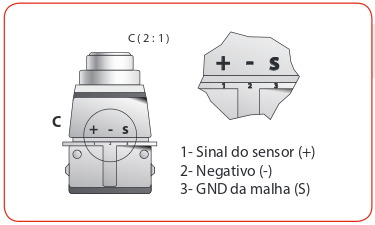
\includegraphics[width=250px, scale=0.5]{figuras/sensor}
    \label{table:patente2}
  \end{figure}
\end{enumerate}
